\documentclass[preview]{standalone}
\usepackage{tikz}

\begin{document}
    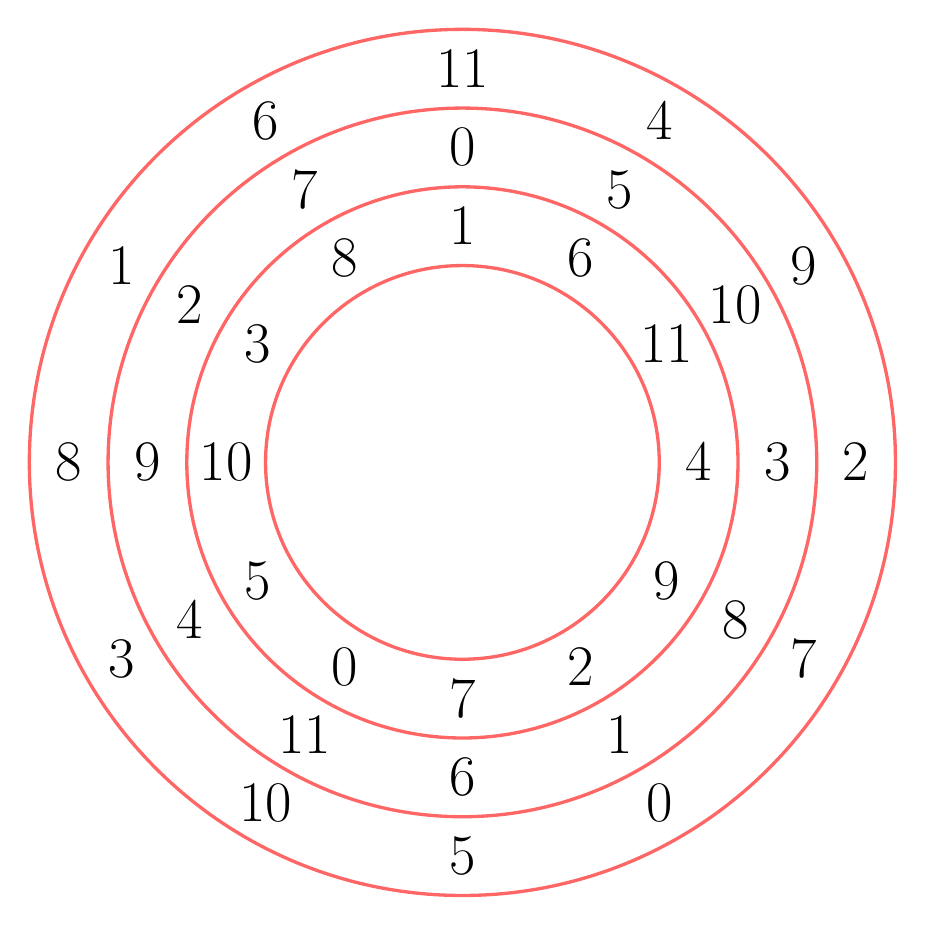
\begin{tikzpicture}
        \def \intervals {{0, 5, 10, 3, 8, 1, 6, 11, 4, 9, 2, 7}}
        \def \names {{"C", "\cdot", "D", "\cdot", "E", "F", "\cdot", "G", "\cdot", "A", "\cdot", "B"}}
        
        \def \n {11}
        \def \max {12}
        
        \def \outerradius {5}
        \def \middleradius {4}
        \def \innerradius {3}
        
       \draw[color=red!60, very thick](0,0) circle (\innerradius - 0.5); 
       \draw[color=red!60, very thick](0,0) circle (\innerradius + 0.5); 
       \draw[color=red!60, very thick](0,0) circle (\middleradius + 0.5); 
       \draw[color=red!60, very thick](0,0) circle (\outerradius + 0.5); 

        
        \def \startangle {-90}

        \foreach \s in {0,...,\n}{
            \pgfmathsetmacro{\angle}{(\startangle - 360/\max*\s}
            
	    \pgfmathsetmacro{\outerlabel}{int(Mod(\intervals[\s] + 11, 12))}
            \pgfmathsetmacro{\middlelabel}{\intervals[\s]}
	    \pgfmathsetmacro{\innerlabel}{int(Mod(\intervals[\s] + 1, 12))}
            
            \draw (\angle:-\outerradius) node {\huge $\outerlabel$};
            \draw (\angle:-\middleradius) node {\huge $\middlelabel$};
            \draw (\angle:-\innerradius) node {\huge $\innerlabel$};
        };

    \end{tikzpicture}
\end{document}
